\clearpage
\thispagestyle{empty} 
\begin{center}
    \vspace*{\fill} 
    \Huge \textbf{Chapter 1} \\
    \Huge \textbf{Security Attacks}
    \vspace*{\fill}
\end{center}
\clearpage

\chapter{Security Attacks}

\section{Definitions and Key Concepts}
\begin{itemize}
    \item \textbf{Security Attack:} Any action compromising the security of information owned by an organization.
    \item \textbf{Security Mechanism:} A process or device designed to detect, prevent, or recover from a security attack.
    \item \textbf{Security Service:} A service that enhances the security of data processing systems and information transfers, countering security attacks using security mechanisms.
\end{itemize}

\section{Threat vs. Attack}
\begin{itemize}
    \item \textbf{Threat:} Any circumstance or event with the potential to adversely impact organizational operations, assets, individuals, or the nation via unauthorized access, destruction, disclosure, modification of information, and/or denial of service.
    \item \textbf{Attack:} Any malicious activity attempting to collect, disrupt, deny, degrade, or destroy information system resources or the information itself.
\end{itemize}

\section{Types of Security Attacks}

\subsection{Passive Attacks}
\begin{itemize}
    \item \textbf{Nature:} Eavesdropping or monitoring transmissions without affecting system resources.
    \item \textbf{Goals:} Obtain information being transmitted.
    \item \textbf{Types:}
    \begin{itemize}
        \item \textit{Release of Message Contents:} Eavesdropping on communications such as phone conversations, emails, or transferred files.
        \item \textit{Traffic Analysis:} Observing the pattern of messages, frequency, and length without examining the contents.
    \end{itemize}
    \item \textbf{Characteristics:} Difficult to detect; prevention usually involves encryption.
\end{itemize}

\subsection{Active Attacks}
\begin{itemize}
    \item \textbf{Nature:} Involves modification of stored or transmitted data or the creation of false data.
    \item \textbf{Types:}
    \begin{itemize}
        \item \textit{Masquerade:} One entity pretends to be another, often combined with other active attacks.
        \item \textit{Replay:} Passive capture and retransmission of data to produce unauthorized effects.
        \item \textit{Data Modification:} Alteration of legitimate messages or reordering/delaying them to produce unauthorized effects.
        \item \textit{Denial of Service:} Preventing or inhibiting normal use or management of communication facilities, either targeting specific entities or disrupting entire networks.
    \end{itemize}
    \item \textbf{Characteristics:} Detection and recovery are primary goals since absolute prevention is difficult.
\end{itemize}

\begin{figure}[h!]
    \centering
    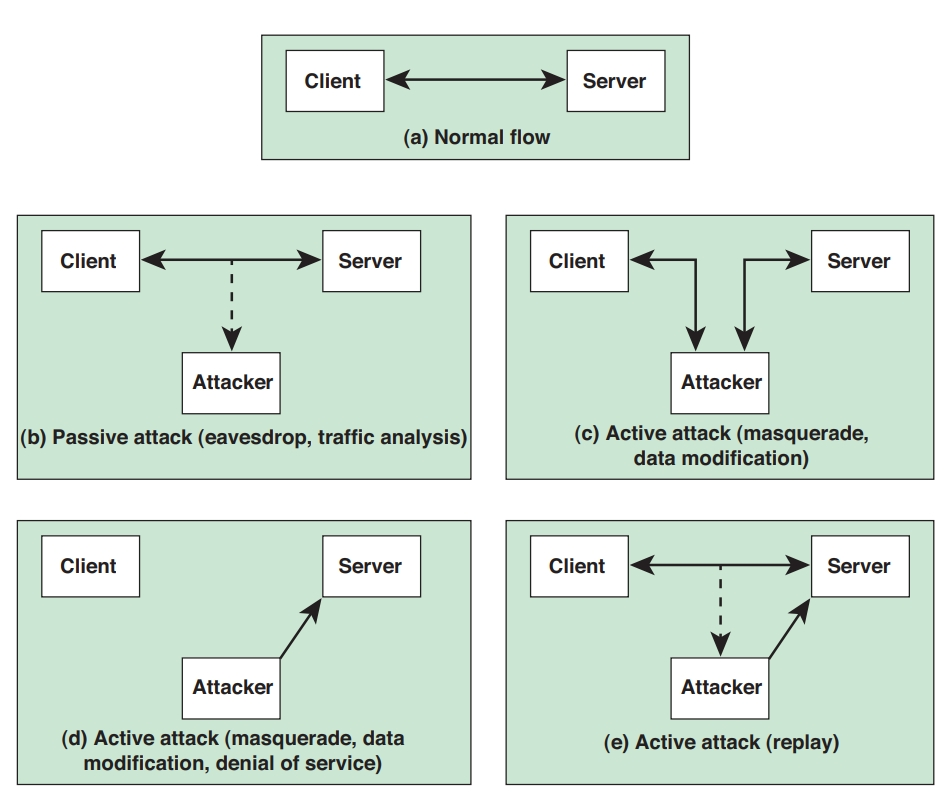
\includegraphics[width=\linewidth]{Data_Privacy_and_Cryptography/Figures/security_attacks.jpeg}
    \caption{Security Attacks}
    \label{fig:security_attacks}
\end{figure}

\section{Illustrations of Security Attacks}
\begin{itemize}
    \item \textbf{Passive Attack Example:} Eavesdropping on client-server communication without disturbing the flow.
    \item \textbf{Active Attack Examples:}
    \begin{itemize}
        \item \textit{Masquerade:} Man-in-the-middle attack, intercepting and pretending to be the client or server.
        \item \textit{Data Modification:} Selectively modifying data communicated between client and server.
        \item \textit{Replay:} Capturing and reusing client messages.
        \item \textit{Denial of Service:} Flooding the server with data or triggering resource-consuming actions.
    \end{itemize}
\end{itemize}
